\section{EINDTOETS · Statistiek, deel 1}

\begin{missie}
Missie: toon wat je kan over steekproeven, misleidingen en causaliteit.
\end{missie}

\textbf{Naam:} \_\_\_\_\_\_\_\_\_\_\_\_\_\_\_\_\_\_\_\_\_\_\_\_\_\_\_\_\_\_ \quad \textbf{Klas:} \_\_\_\_\_\_\_\_\_\_\_\_\_ \quad \textbf{Datum:} \_\_\_\_\_\_\_\_\_\_\_\_\_

\textbf{Hulpmiddelen:} rekentoestel of Excel/GeoGebra. \quad \textbf{Duur:} ongeveer 60 minuten. \quad \textbf{Totaal:} 60 punten.

\begin{letop}
\textbf{Zo werk je:} schrijf je werkwijze op en eindig bij contextvragen met een antwoordzin. Rond percentages af op 0,1 \% tenzij anders vermeld.
\end{letop}

\textbf{Doelenmatrix}

\breedtes{52/24/24}
\begin{tabular}{lcc}
\hline
Doel & Vragen & Punten \\
\hline
Statistisch onderzoek en variabelen (basis) & 1 – 3 & 12 \\
LPD 11: populatie, steekproef, steekproefvariabiliteit, representativiteit, steekproefontwerp & 4 – 9 & 22 \\
LPD 1 – 3: misleidingen beschrijven, problemen oplossen, ICT & 10 – 12 & 12 \\
LPD 12: samenhang en causaliteit, onderzoeksopzet & 13 – 15 & 14 \\
LPD 4: redenering uitleggen & verweven in 7, 8, 10, 15 & \\
\hline
\end{tabular}

\subsection*{A · Statistisch onderzoek en variabelen}

\textbf{Vraag 1 \quad (4 p)} Zet de stappen van een onderzoek in de juiste volgorde.

\textbf{A} De resultaten worden besproken met de ouders. \quad \textbf{B} De kinderopvang merkt dat veel kinderen te weinig slapen. \quad \textbf{C} De antwoorden worden verwerkt in tabellen en grafieken. \quad \textbf{D} De ouders vullen een vragenlijst in. \quad \textbf{E} Men stelt de onderzoeksvraag ‘Hoeveel uur slapen de kinderen?’ \quad \textbf{F} Men besluit dat de meeste kinderen minder dan tien uur slapen.

Volgorde: \_\_ – \_\_ – \_\_ – \_\_ – \_\_ – \_\_

\begin{oplossing}
\textbf{Oplossing 1} \quad B – E – D – C – F – A. (4 p: 4 punten bij volledig correct; 3 p bij één omwisseling; 2 p bij twee; 1 p bij drie juist geplaatste stappen.)
\end{oplossing}

\textbf{Vraag 2 \quad (4 p)} Een zorgorganisatie bevraagt haar medewerkers. Noteer de onderzochte variabele en zet een kruisje als ze kwantitatief is.

\breedtes{50/32/18}
\begin{tabular}{lll}
\hline
Enquêtevraag & Variabele & Kwantitatief? \\
\hline
a) Hoeveel uur werk je per week? & & \\
b) Hoe tevreden ben je over je team? (zeer ontevreden – … – zeer tevreden) & & \\
c) In welke afdeling werk je? & & \\
d) Hoeveel minuten ben je per dag onderweg naar het werk? & & \\
\hline
\end{tabular}

\begin{oplossing}
\textbf{Oplossing 2} \quad a) aantal gewerkte uren per week (x) b) tevredenheid over het team c) afdeling d) reistijd in minuten per dag (x). (1 p per rij)
\end{oplossing}

\textbf{Vraag 3 \quad (4 p)} Een school met 800 leerlingen vraagt aan 100 geloote leerlingen hoeveel uur ze per week sporten.

\textbf{a)} Noteer de populatie, de steekproef, $N$ en $n$. (2 p) \lijn

\textbf{b)} Noteer de variabele en het soort variabele en data. (2 p) \lijn

\begin{oplossing}
\textbf{Oplossing 3} \quad a) populatie: alle 800 leerlingen ($N=800$); steekproef: de 100 geloote leerlingen ($n=100$) (2). b) aantal uur sport per week; kwantitatief, numerieke data (2).
\end{oplossing}

\subsection*{B · Steekproef en populatie (LPD 11)}

\textbf{Vraag 4 \quad (3 p)} Geef drie verschillende redenen waarom men met een steekproef werkt in plaats van met de hele populatie. \lijn

\begin{oplossing}
\textbf{Oplossing 4} \quad Te duur; te veel tijd; ethische redenen; het onderzoek vernietigt het product/de populatie; onmogelijk om iedereen te bereiken. (1 p per reden, max. 3)
\end{oplossing}

\textbf{Vraag 5 \quad (3 p)} Twee scholen trekken elk een steekproef van 50 leerlingen en vragen hoeveel uur ze slapen. School A vindt een gemiddelde van 7,4 uur, school B 7,9 uur.

\textbf{a)} Verklaar waarom de gemiddelden verschillen. (2 p) \lijn

\textbf{b)} Wat verwacht je als beide scholen steekproeven van 500 leerlingen trekken? (1 p) \lijn

\begin{oplossing}
\textbf{Oplossing 5} \quad a) Steekproefvariabiliteit: andere leerlingen, dus andere resultaten (2). b) De gemiddelden liggen dichter bij elkaar en bij het populatiegemiddelde (1).
\end{oplossing}

\textbf{Vraag 6 \quad (3 p)} Koppel: schrijf V (verzamelende), B (beschrijvende) of K (verklarende) statistiek.

\textbf{a)} Een onderzoeksbureau laat 500 ouders een vragenlijst invullen. \_\_ \quad \textbf{b)} De antwoorden worden samengevat in een tabel en een staafdiagram. \_\_ \quad \textbf{c)} Men besluit: ‘De meeste Vlaamse ouders vinden de opvang betaalbaar.’ \_\_

\begin{oplossing}
\textbf{Oplossing 6} \quad a) V \quad b) B \quad c) K (1 p elk)
\end{oplossing}

\textbf{Vraag 7 \quad (5 p)} Zet een kruisje bij elk criterium voor een representatieve steekproef dat niet vervuld is: (1) omvang voldoende groot, (2) samenstelling komt overeen met de populatie, (3) non-respons niet te groot. Leg telkens kort uit.

\breedtes{58/10/10/10}
\begin{tabular}{llll}
\hline
Situatie & 1 & 2 & 3 \\
\hline
a) Een stad met 120\,000 inwoners baseert zich op een bevraging van 30 inwoners. & & & \\
b) Van de 300 uitgenodigde ouders vullen er 21 de vragenlijst in. & & & \\
c) Een onderzoek naar werkdruk bevraagt enkel verpleegkundigen van één groot stadsziekenhuis, 40 personen. & & & \\
\hline
\end{tabular}

\begin{oplossing}
\textbf{Oplossing 7} \quad a) criterium 1 (30 is veel te weinig) (1). b) criterium 3 (responspercentage $\frac{21}{300}=7\,\%$) (1). c) criteria 1 en 2 (40 personen en alleen een stedelijk ziekenhuis, geen thuiszorg of woonzorgcentra) (3 p: 1 per kruisje, 1 voor uitleg).
\end{oplossing}

\textbf{Vraag 8 \quad (4 p)}

\textbf{a)} Wat is een enkelvoudig aselecte steekproef? (1 p) \lijn

\textbf{b)} Beschrijf hoe je een EAS van 60 jongeren trekt uit 1\,200 jongeren van een jeugdbeweging. (2 p) \lijn

\textbf{c)} Waarom is zo’n steekproef waarschijnlijk representatief? (1 p) \lijn

\begin{oplossing}
\textbf{Oplossing 8} \quad a) Elk element van de populatie heeft dezelfde kans om gekozen te worden, door volledig willekeurige trekking (1). b) Elke jongere een nummer 1 – 1\,200 geven (1) en met de computer lukraak 60 verschillende nummers trekken (1). c) Geen groep is bevoordeeld door toeval; bij voldoende omvang weerspiegelt de steekproef de populatie (1).
\end{oplossing}

\textbf{Vraag 9 \quad (4 p)} Welke vorm van vertekening is het: opportunistisch of vrijwillige respons? Verklaar kort.

\textbf{a)} Een leerling bevraagt enkel de mensen in de wachtzaal van de huisarts naast school. \lijn

\textbf{b)} Een zender vraagt kijkers om te stemmen via sms op de vraag ‘Is de speeltijd te kort?’. \lijn

\begin{oplossing}
\textbf{Oplossing 9} \quad a) opportunistisch (gemakkelijk bereikbare mensen) (2). b) vrijwillige respons (wie wil, stemt; vooral uitgesproken meningen) (2).
\end{oplossing}

\subsection*{C · Misleidingen en valkuilen (LPD 1 – 3)}

\textbf{Vraag 10 \quad (5 p)} Een jeugdkamp publiceert deze grafiek.

\begin{center}
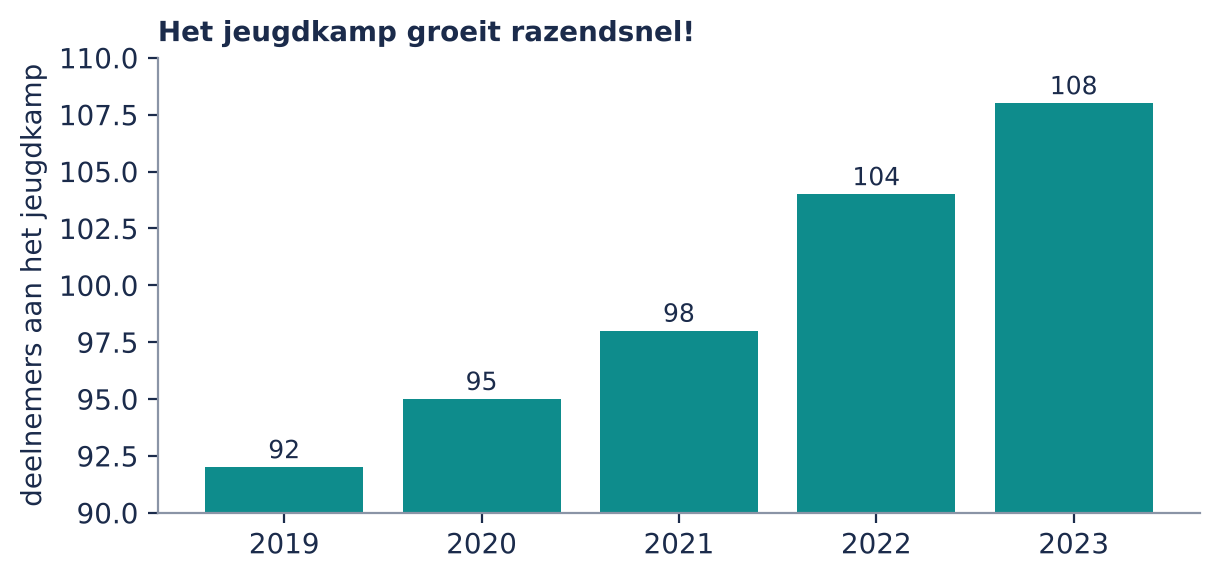
\includegraphics[width=0.7\textwidth]{figuren/d1_toets_staaf.png}
\end{center}

\textbf{a)} Welke misleiding zie je en wat is het misleidende gevolg? (2 p) \lijn

\textbf{b)} Bereken met ICT met hoeveel procent het aantal deelnemers steeg van 2019 tot en met 2023. (2 p) \lijn

\textbf{c)} Hoe zou je de grafiek wel eerlijk maken? (1 p) \lijn

\begin{oplossing}
\textbf{Oplossing 10} \quad a) De verticale as begint bij 90 in plaats van bij 0 (1); het lijkt of het aantal deelnemers verschillende keren is gestegen, terwijl de stijging beperkt is (1). b) $\frac{108-92}{92}\approx 0{,}174=17{,}4\,\%$ (2). c) De verticale as laten beginnen bij 0 (1).
\end{oplossing}

\textbf{Vraag 11 \quad (4 p)} Het aandeel jongeren dat dagelijks een uur sport, stijgt van 25 \% naar 40 \%. Daarna daalt het van 80 \% naar 60 \% in een andere groep.

\textbf{a)} Geef de stijging van 25 \% naar 40 \% in procentpunt en in procent. (2 p) \lijn

\textbf{b)} Geef de daling van 80 \% naar 60 \% in procentpunt en in procent. (2 p) \lijn

\begin{oplossing}
\textbf{Oplossing 11} \quad a) 15 procentpunt (1); $\frac{40-25}{25}=0{,}60=60\,\%$ (1). b) 20 procentpunt (1); $\frac{60-80}{80}=-0{,}25$, dus 25 \% daling (1).
\end{oplossing}

\textbf{Vraag 12 \quad (3 p)} De maandlonen (in euro) van zeven medewerkers van een opvang: 2\,300 – 2\,350 – 2\,400 – 2\,450 – 2\,500 – 2\,600 – 7\,000.

\textbf{a)} Bereken met ICT het gemiddelde en de mediaan. (2 p) \lijn

\textbf{b)} Wie zal het gemiddelde gebruiken en wie de mediaan als het over de lonen gaat? (1 p) \lijn

\begin{oplossing}
\textbf{Oplossing 12} \quad a) $\overline{x}=\frac{21\,600}{7}\approx 3\,085{,}7$ euro (1); Med = 2\,450 euro (1). b) De directie gebruikt het gemiddelde (hoger), de vakbond de mediaan (de uitschieter 7\,000 euro trekt het gemiddelde omhoog) (1).
\end{oplossing}

\subsection*{D · Samenhang en causaliteit (LPD 12)}

\textbf{Vraag 13 \quad (4 p)} Welke misvatting zit er in elke uitspraak: omgekeerde richting (O), toeval (T) of derde variabele (D)?

\textbf{a)} Mensen die dagelijks naar een therapeut gaan, zijn gemiddeld ongelukkiger. Therapie maakt ongelukkig. \_\_

\textbf{b)} Kinderen met veel speelgoed halen betere punten. Speelgoed zorgt dus voor betere punten. Leg uit. \_\_ \lijn

\textbf{c)} Het aantal ooievaars en het aantal geboortes in regio’s stijgen samen. Ooievaars brengen baby’s. \_\_

\begin{oplossing}
\textbf{Oplossing 13} \quad a) O (1). b) D (1): bv. het inkomen of de betrokkenheid van de ouders beïnvloedt beide (1). c) D (landelijke gebieden) of T (1).
\end{oplossing}

\textbf{Vraag 14 \quad (5 p)} Een school loot 300 leerlingen in een groep met en een groep zonder een buddyproject (150 + 150). Na een jaar kijkt men of het aantal pestincidenten verminderde, gelijk bleef of toenam.

\breedtes{28/18/18/18/18}
\begin{tabular}{lcccc}
\hline
 & verminderd & gelijk & toegenomen & totaal \\
\hline
buddyproject & 90 & 45 & 15 & \\
controlegroep & 50 & 70 & 30 & \\
totaal & & & & \\
\hline
\end{tabular}

\textbf{a)} Vul de tabel aan. (1 p) \lijn

\textbf{b)} Bereken het percentage leerlingen bij wie het pesten verminderde, in elke groep. (2 p) \lijn

\textbf{c)} Is dit observationeel of experimenteel? Mag je causaliteit besluiten? Verklaar. (2 p) \lijn

\begin{oplossing}
\textbf{Oplossing 14} \quad a) Totalen: 150, 150; 140 – 115 – 45 – 300 (1). b) Buddyproject: $\frac{90}{150}=60{,}0\,\%$; controlegroep: $\frac{50}{150}\approx 33{,}3\,\%$ (2). c) Experimenteel (de school grijpt in en verdeelt de leerlingen door loting) (1); omdat de groepen willekeurig zijn samengesteld, is het verschil waarschijnlijk te wijten aan het project: een causaal verband is mogelijk (1).
\end{oplossing}

\textbf{Vraag 15 \quad (5 p)} Een vitaminebedrijf meldt: ‘Uit een bevraging van 800 abonnees van onze nieuwsbrief blijkt dat 9 op 10 ouders die hun kind dagelijks vitamines geven, zelden ziek zijn. Vitamines beschermen tegen ziekte!’ De bevraging werd betaald door het bedrijf.

\textbf{a)} Noteer drie problemen met deze uitspraak en benoem ze met begrippen uit deze bundel. (3 p) \lijn

\textbf{b)} Hoe zou je kunnen onderzoeken of vitamines kinderen beschermen? (2 p) \lijn

\begin{oplossing}
\textbf{Oplossing 15} \quad a) Opportunistische steekproef/vrijwillige respons (abonnees die reageren) = niet representatief (1); de opdrachtgever is het bedrijf (1); samenhang wordt gelezen als causaliteit, een derde variabele (gezonde levensstijl) of omgekeerde richting is mogelijk (1). b) Experiment: kinderen door loting verdelen in een groep met vitamines en een controlegroep (placebo), zelfde omstandigheden, na enkele maanden het aantal ziektedagen vergelijken (2).
\end{oplossing}

\begin{doel}
\textbf{Mijn score:} \_\_\_\_ / 60 \quad \textbf{Behaald vanaf 36 / 60 (60 \%).}

Per onderdeel: Basis \_\_ / 12 \quad LPD 11 \_\_ / 22 \quad LPD 1 – 3 \_\_ / 12 \quad LPD 12 \_\_ / 14
\end{doel}
